%=====================================================================
\section{Experiments}
\label{sec:experiments}
%=====================================================================

We test whether the standard protocol can tell erasing a concept from destroying its words, how \cinder{} compares with \ember{} under a collateral-aware evaluation, and whether one \cinder{} fit can replace per-language \ember{}.

\subsection{Experimental Setup}
\label{sec:setup}

\paragraph{Models and Data}
We use Gemma-2-2B-it \citep{gemma2024gemma2} in English and Llama-3.1-8B-Instruct \citep{grattafiori2024llama3} in eight languages.
As in \ember{}, $\Sc$ and $\Sn$ hold 300 Wikipedia sentences each, with 50 validation and 50 test questions per concept.
We developed the evaluation on Harry Potter, Ancient Rome and Valentine's Day and test on \expnum{12} of \ember{}'s other concepts with 5 seeds each (\expnum{60} runs); the multilingual study uses \ember{}'s 18 concepts and 20 new ones held out under a pre-registered protocol (\S\ref{app:ml}).

\paragraph{Evaluation Metrics}
We keep \ember{}'s metrics except relearning (\S\ref{sec:prelim}) and add two that target the edited tokens; the multilingual study keeps \ember{}'s alone, with perplexity on native text in place of Alpaca.
\emph{Collateral} is accuracy on multiple-choice questions that use an edited token outside the concept, such as \emph{Harry} in Prince Harry or \emph{Caesar} in Caesar salad (\expnum{3{,}501} items on \expnum{1{,}026} tokens), written by LLM agents blind to the methods and frozen before any edited model was scored.
\emph{Word integrity} tests whether the model can still copy, define and read past an edited word, and keep its answers on neutral prompts that use it, against two references: the word deleted, and a \emph{nonce}, a pronounceable non-word that the model can repeat but does not understand, which is how an erased word should behave.
Operating points are selected by $\Hthree = \hmean(\text{efficacy}, \text{specificity}, \text{collateral})$ among points that keep MMLU and collateral above 0.9 and 0.8 of the unedited model.
Since equal $\delta$ does not mean equal edits across methods, all methods sweep one grid of \emph{edit sizes} $r = \operatorname{median}_t \|\e_t' - \e_t\| / \|\e_t\| \in \{0.05, \dots, 100\}$, where $r = 1$ means that each edit is as long as the token.
As all questions are fixed in advance, scoring a grid point needs only forward passes, whereas \ember{}'s coherence term calls an LLM judge on 150 Alpaca outputs per point (\S\ref{app:eval}).

\paragraph{Methods and Statistics}
We compare \ember{}, \cinder{} (\cs{} + \gs{} + \twj{}), \cinderz{} and, to isolate Global Sparsity (\gs{}), \cinder{}-RS and \cinder{}-RS-z with row sparsity; in the multilingual study, A1 runs \ember{} per language, A2 is one multilingual \ember{} fit, A3 is multilingual \cinder{}, and A3z its \cinderz{} edit.
Each method selects one operating point per run on validation questions (besides our rule, we report \ember{}'s $H$ without Alpaca and a fixed $r = 0.5$) and is scored once on test questions.
Comparisons are paired by run, with the concept as the unit (Wilcoxon tests, Holm correction, bootstrap 95\% intervals); only the comparisons under our rule, $H$ and fixed $r$ and the multilingual hypotheses (\S\ref{app:ml}) were pre-registered, and other analyses are post hoc unless marked.

\subsection{Results}
\label{sec:results}

\paragraph{The standard protocol rewards token destruction}
Without a collateral term, selection settles on edits a hundred times the token's length for \ember{} and \cinderz{} (Table~\ref{tab:destruction}); with it, every method moves to $r \approx 1$.
At the destructive points, \expnum{24--34\%} of neutral prompts break, and efficacy exceeds the level reached by deleting the edited words from the questions (\expnum{0.23--0.28}) in \expnum{83\%} and \expnum{98\%} of runs: the edits likely derail the prompt as well as delete the word.
Alpaca coherence registers none of this, and under $H$ the ranking reappears through destruction, with \ember{} ahead of \cinder{} (n.s.).

\begin{table}[t]
  \centering
  \small
  \setlength{\tabcolsep}{3pt}
  \begin{tabular}{@{}lccccc@{}}
    \toprule
    Method, rule & $r$ & Eff.$\uparrow$ & Coll.$\uparrow$ & Broken$\downarrow$ & Alp.$\uparrow$ \\
    \midrule
    \ember{}, $H$ & \expnum{100} & \expnum{0.47} & \expnum{0.73} & \expnum{0.24} & \expnum{0.97} \\
    \ember{}, $\Hthree$ & \expnum{1} & \expnum{0.29} & \expnum{0.85} & \expnum{0.15} & \expnum{0.97} \\
    \cinderz{}, $H$ & \expnum{100} & \expnum{0.68} & \expnum{0.68} & \expnum{0.34} & \expnum{0.97} \\
    \cinderz{}, $\Hthree$ & \expnum{1} & \expnum{0.39} & \expnum{0.86} & \expnum{0.16} & \expnum{0.98} \\
    \bottomrule
  \end{tabular}
  \caption{Points selected by \ember{}'s $H$ (without Alpaca) and our $\Hthree$ on 12 held-out concepts (test). Broken: neutral prompts whose answer breaks (9 concepts, one seed); Alp.: Alpaca coherence (seed 42).}
  \label{tab:destruction}
\end{table}

\paragraph{\cinder{} erases concepts that \ember{} misses}
\ember{} edits in \expnum{41} of the 60 held-out runs and \cinder{} in \expnum{52}; in runs where only one of them edits, \cinder{} does so in \expnum{14} and \ember{} in \expnum{3} (run-level exact McNemar $p = \expnum{0.013}$, post hoc).

\paragraph{At moderate edit size, \cinder{}'s direction removes more}
At $r = 0.5$, every \cinder{} variant removes more than \ember{} at the same collateral (efficacy \expnum{0.25--0.30} vs.\ \expnum{0.20}); for \cinder{}, the gain is \expnum{$+0.15$} $\Hthree$ on \expnum{10 of 11} concepts (Holm $p = \expnum{0.012}$; Figure~\ref{fig:results}).
Crossing the two token sets with the two directions (post hoc) attributes it to the direction (\expnum{$+0.07$} efficacy, \expnum{10 of 11} concepts, Holm $p = \expnum{0.10}$) rather than the token set (\expnum{$+0.02$}; \S\ref{app:dir}).
At $r = 1$ it vanishes (\expnum{$-0.02$}, $p = \expnum{0.97}$; post hoc): on the development concepts, centred directions plateau near the deletion floor by then, and \ember{} passes it only by damaging the prompt (\S\ref{app:mean}).

\paragraph{At their own operating points, the methods tie}
When each method picks its own strength, the pre-registered primary comparison shows no significant difference (\expnum{$+0.04$}, Holm $p = \expnum{0.41}$): both settle near $r = 1$, where the direction effect vanishes.
With a stricter collateral gate (0.9), all four \cinder{} variants beat \ember{} significantly, though not with a looser one (0.7; post hoc; \S\ref{app:eval}).

\begin{figure}[t]
  \centering
  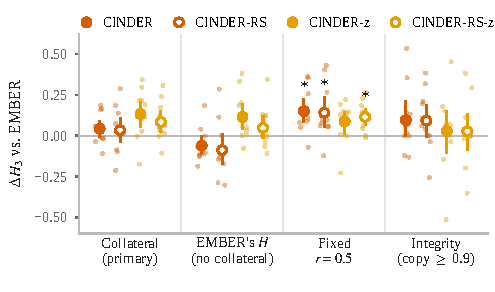
\includegraphics[width=\columnwidth]{figures/results.pdf}
  \caption{Paired test $\Hthree$ difference to \ember{} on the 11 held-out concepts where both edit, by selection rule (integrity-gated: copy $\geq 0.9$, post hoc). Dots: concepts; bars: 95\% bootstrap CI; $*$: Holm $p < 0.05$.}
  \label{fig:results}
\end{figure}

\subsection{Multilingual Erasure}
\label{sec:exp-ml}

\paragraph{One \cinder{} fit replaces eight \ember{} fits}
Counting concepts without an edit as failures, the single \cinderz{} fit (A3z) ties per-language \ember{} (A1; exploratory, non-inferiority not shown): \expnum{0.23} vs.\ \expnum{0.25} strict and \expnum{0.28} vs.\ \expnum{0.25} ungated, \expnum{15--13} in wins and losses ($p = \expnum{0.78}$; Table~\ref{tab:ml}).
Pooling three fit seeds helps \cinderz{} (\expnum{$+0.08$}, $p < 0.001$) but not per-language \ember{}, and the two still tie.

\begin{table}[t]
  \centering
  \small
  \setlength{\tabcolsep}{3.5pt}
  \begin{tabular}{@{}lcccc@{}}
    \toprule
     & A1 & A2 & A3 & A3z \\
    \midrule
    Fits per concept & 8 & 1 & 1 & 1 \\
    Judge calls per concept & \expnum{160} & \expnum{20} & \expnum{20} & \expnum{20} \\
    LLM cost per concept (NIS) & \expnum{.055} & \expnum{.007} & \expnum{.017} & \expnum{.017} \\
    Concepts with a feature (of 38) & \expnum{26} & \expnum{10} & \expnum{21} & \expnum{21} \\
    Score, strict & \expnum{0.25} & \expnum{0.11} & \expnum{0.14} & \expnum{0.23} \\
    Score, ungated & \expnum{0.25} & \expnum{0.14} & \expnum{0.14} & \expnum{0.28} \\
    \bottomrule
  \end{tabular}
  \caption{Multilingual erasure on Llama-3.1-8B-Instruct (38 concepts, 8 languages, fit seed 42, test split; approaches in \S\ref{sec:setup}); concepts without an edit score 0.}
  \label{tab:ml}
\end{table}

\paragraph{A multilingual \ember{} fit rarely accepts the concept}
Where the multilingual \ember{} fit (A2) selects a concept feature, it erases as well as \cinderz{}, but it does so for only \expnum{10} of 38 concepts and \expnum{2} of the 20 held-out ones, against \expnum{21} and \expnum{10} for \cinder{}; counting coverage, \cinderz{} beats it by \expnum{$+0.21$} (\expnum{15--4}, $p = \expnum{0.011}$).
The loss is at the judge more than in the fit: the raw fit contains a lexicon-matching concept feature about as often as \cinder{}'s (\expnum{25--27} vs.\ \expnum{23--28} concepts per seed), but \ember{}'s judge accepts only \expnum{5\%} of those with 3--4 lexicon words, against \expnum{30\%} for \cinder{}'s; re-judged, \twj{} alone lifts the raw fit from \expnum{10} to \expnum{18} concepts, and sharpening alone to \expnum{16} (seed 42, post hoc; \S\ref{app:ml}).

\paragraph{The mean term matters across languages}
Multilingual \cinder{} (A3), whose edit is centred, erases weakly; its uncentred edit (A3z, defined after the development results) adds \expnum{$+0.17$} (\expnum{16 of the 21} edited concepts, $p = \expnum{0.007}$), in the same direction on the 20 pre-registered held-out concepts (\expnum{$+0.19$}, \expnum{7--3}, $p = \expnum{0.064}$).
Across all approaches, erasure is strongest in English, about 0.6 of that in the other Latin-script languages, little in Thai and almost none in Hindi, whose words split into pieces that are rarely concept-only (\S\ref{app:ml}).
